\documentclass[11pt, a4paper]{article}

\usepackage{enumitem}
\usepackage{mathtools}
\usepackage{hyperref}
\usepackage{tikz}
%\usepackage[top=1in, bottom=0.4in]{geometry}

\pagenumbering{gobble}

\begin{document}

  \title{Addressing cold start in music recommendation}
  \author{Ioannis Gakos, Wiktor Grajkowski - Group 37}
  \date{16th April 2016}
  \maketitle

  \section{Introduction}
    The shift of the music industry towards the Web has made music
    recommendation a relevant problem which solution could radically improve
    users' experience. However, in the absence of usage data, existing methods,
    such as collaborative filtering, fall short in taking effective decisions
    for new and unpopular content.
    \\ \\
    \noindent
    This project aims to build a music recommendation system using
    Convolutional Neural Network (CNN). CNNs have been widely used in
    applications such as image recognition and recommendation systems. Our
    design is based on recent work of Aaron van den Oord et al. on music
    recommendation \cite{deep-content-based-music-recommendation} using deep
    CNNs and on Dieleman's post \cite{spotify-dieleman} on the implementation
    and architecture details of such CNN built during his internship at
    Spotify.
    \\ \\
    \noindent
    Our main objective is to build a system that addresses the cold start
    problem for both new users and music content. The users give a single
    preferred track as input, based on which a shuffled playlist with similar
    music is generated. Newly imported music content, without previous usage
    related feedback, can be classified based solely on its frequency spectrum.
    It is achieved by propagating the spectrum through a CNN trained to predict
    latent representations obtained from a separate, tag based model. The tags
    and audio samples were obtained from MagnaTagATune open dataset consisting
    of 26,000 user annotated audio clips.

  \section{Problem}
    Traditional content recommendation systems rely on user usage data to make
    decisions. Behavior patterns between users, are used by collaborative
    filtering methods to make recommendations about various types of content.
    However, collaborative filtering suffers from the cold start problem.
    Latent factor vectors are compact representations of the user's preferences
    correlated with other characteristics of the items. Predicting these
    vectors for new music content based only on metadata such as the artist's
    name is often impossible. Using audio content to predict latent factor
    vectors can bridge the semantic gap between the characteristics of an audio
    track and the user's preferences. A\"{a}ron van den Oord et al. converted
    existing usage data, present in the MagnaTagATune dataset, to the latent
    vector space using Weighted Matrix Factorization and trained a CNN using
    these vectors to minimize the Mean Squared Error of the predicted latent
    vectors of audio samples. Visualization of their qualitative evaluation is
    depicted in Figure 1.

    \begin{figure}
      \centering
      \rotatebox{0}{\scalebox{1}{
        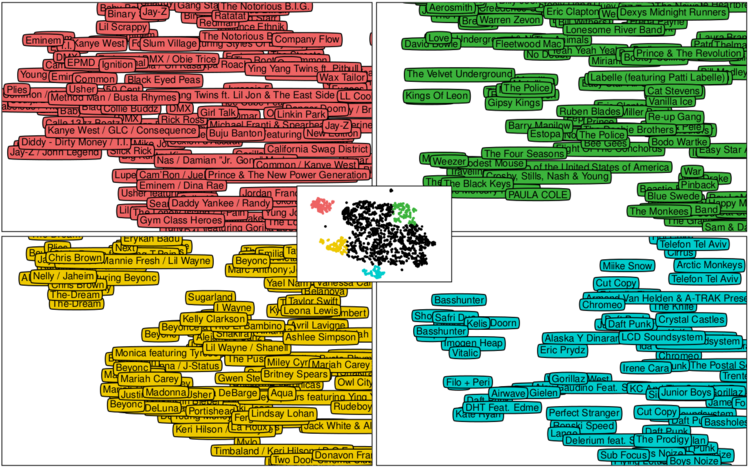
\includegraphics[
          width=12cm,height=12cm,keepaspectratio]{latent-space-visualization.png}}}
      \caption{Visualization of the artist classification using latent factors
        predicted from audio (
        \url{http://benanne.github.io/images/prentje\_nips.png})}
    \end{figure}

  \section{Related Work}
  \section{About the dataset}
    In order to train the CNN, we are using the MagnaTagATune dataset, which
    was made available by the Magnatune label for the research community. The
    data was collected using the TagATune game where users annotated audio
    tracks with audio relevant tags.
    \\ \\
    \noindent
    The dataset consists of approximately 26,000 of 29 seconds music clips
    encoded in 16 kHz, 32kbps, mono mp3, generously contributed by John
    Buckman, the founder of every MIR researcher's favorite label Magnatune.
    Each of them is annotated with a combination of 188 tags such as
    "orchestral", "orchestra", "punk", "slow", "blues", "rock" etc. It also
    contains music similarity annotations in the form of triples where given a
    triple of songs (A, B, C), metrics of how many players have flagged the
    song A, B or C as most different from the others. \cite{msd-dataset}

  \section{Design architecture}
    Our system needs to be able to suggest songs similar to that provided by
    the user, based only on its audio sample. To achieve this goal we first
    build a ground truth model using MagnaTagATune dataset. Each song in the
    database is annotated by users with multiple tags that we treat as ``bag of
    words'' meaning only the presence and count of a tag matters and but its
    position. We will run word2vec algorithm using gensim Python toolkit on
    this dataset to produce latent vector representation of each song. We will
    then build a Convolutional Neural Network taking frequency spectrum of an
    audio sample as input and outputting latent vector representation. The
    Network will be trained to minimize the MSE of the predictions with the
    ground truth model. We will use compressed mel-spectograms of the audio
    samples to form compressed time-frequency representations and use them to
    train our CNN. The samples will overlap in time. We will experiment with
    the depth and size of the network. Figure 2 shows possible configuration
    with three convolutional layers and three fully connected layers.

    \begin{figure}
      \centering
      \rotatebox{0}{\scalebox{1}{
        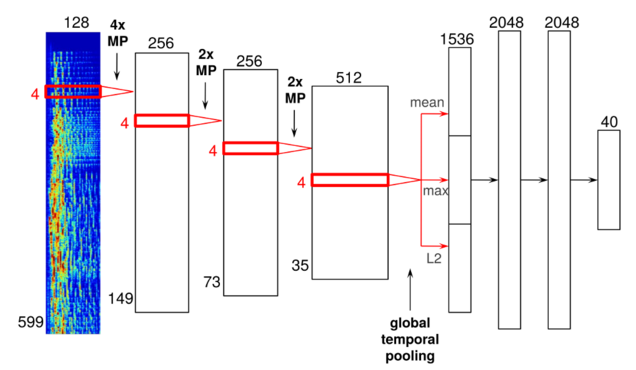
\includegraphics[
          width=12cm,height=12cm,keepaspectratio]{cnn-architecture.png}}}
      \caption{One of the convolutional neural network architectures Dieleman
        experimented with, on which our design decisions are based as well
        (\url{ http://benanne.github.io/images/spotify\_convnet.png}).}
    \end{figure}

  \section{Implementation Details}
    In order to facilitate building and training the Convolutional Neural
    Network we used the Lasagne, the most mature and active lightweight library
    currently available in the community \cite{lasagne}. The library provides
    already implemented layers such as 2D Convolutional and Fully connected
    ones (DenseLayer) that we used in our implementation.
    \\ \\
    \noindent
    Before training the network, we applied a lot of preprocessing on the
    dataset we used resulting in a dataset of 21642 training, validation and 
    testing samples. The preprocessing included exclusion of samples from the
    dataset that had no tags attached in order to avoid pushing the training
    towards overfitting on tracks with no feature information available.
    \\ \\
    \noindent
    To move from tags to the latent vector space and this way build the ground
    truth model, we used the Doc2Vec model that the network used to minimize
    its predictions' error \cite{doc2vec}. In order to prepare samples for
    training we used the librosa library \cite{librosa} to extract the mel
    spectrograms of all of the samples included in the dataset, a rather time
    consuming process.
    \\ \\
    \noindent
    Our implementation provides a full working flow, meaning that it supports
    all the steps from preprocessing the dataset up to the point of getting
    a list of the 10 most similar tracks given as target a track from the
    dataset. It also supports multiple execution environments based on the
    computational power available. We did that because we needed to be able to
    quickly switch from our local development environments to the production
    one that we used for training, an EC2 instance equipped with a GPU in AWS.
      
  \section{Tests and Results}

  \section{Time Constraints}
  \section{Discussion}
    Being able to classify music in the latent vector space without having
    usage data, can help companies in the industry of digital music
    distribution take more sophisticated decisions for new audio content.
    Having Dieleman's prototype description will help us make comparisons based
    on the evaluation results of both systems, for example concerning the
    granularity of the filters learnt. We expect the problem to be challenging
    enough, especially when it comes on adjusting the overlapping samples in
    various time frame sizes and deciding on the exact CNN layer architecture,
    for example how many fully connected layers does our model need.
  \section{Conclusion}
    We believe we approached the problem of cold start for music recommendation
    the right way, by training a CNN to learn filters based on the frequency
    spectrum of a track and its representation in the latent vactor space. In
    the interest of time and computational resources available, we had to make
    a lot of compromises with the most effective one being the used dataset.
    Though being a great resource, the MagnaTagATune dataset seems not to
    include enough samples for the model to learn a great variety of filters.
    Going for larger datasets like the 1 Million Song dataset was definitely
    not a reasonable option, as a full training session for such a dataset
    would take days instead of several hours that our model did.

  \begin{thebibliography}{9}
    \sf
    \bibitem{deep-content-based-music-recommendation}
      Aaron van den Oord, Sander Dieleman, Benjamin Schrauwen, \emph{``Deep
      content-based music recommendation''}
    \bibitem{deep-learning-signal-processing}
      Deng, Li, and Dong Yu. \emph{"Deep learning: Methods and applications."}
      Foundations and Trends in Signal Processing 7.3–4 (2014): 197-387.
    \bibitem{spotify-dieleman}
      Sander Dieleman, \emph{Recommending music on Spotify with deep learning},
      \url{http://benanne.github.io/2014/08/05/spotify-cnns.html}
    \bibitem{hamel-temp-pooling}
      Hamel, Philippe, et al. \emph{TEMPORAL POOLING AND MULTISCALE LEARNING
      FOR AUTOMATIC ANNOTATION AND RANKING OF MUSIC AUDIO}.
    \bibitem{msd-dataset}
      Thierry Bertin-Mahieux, Daniel P.W. Ellis, Brian Whitman, and Paul
      Lamere. \emph{The Million Song Dataset}. In Proceedings of the 12th
      International Society for Music Information Retrieval Conference (ISMIR
      2011), 2011.
    \bibitem{cs231n}
      CS231n Convolutional Neural Networks for Visual Recognition,
      \url{http://cs231n.github.io/}
    \bibitem{lasagne}
      Lasagne, \url{https://github.com/Lasagne/Lasagne}
    \bibitem{doc2vec}
      Doc2Vec, gensim \url{https://radimrehurek.com/gensim/models/doc2vec.html}
    \bibitem{librosa}
      librosa, \url{https://github.com/bmcfee/librosa}
  \end{thebibliography}
\end{document}
